\documentclass[11pt]{article}
\usepackage[margin=1in]{geometry}
\usepackage{newtxtext,newtxmath}
\usepackage{booktabs,graphicx,caption,subcaption,xcolor,hyperref,listings,enumitem,array}
\usepackage[T1]{fontenc}
\hypersetup{colorlinks=true,linkcolor=blue!50!black,urlcolor=blue!50!black,citecolor=blue!50!black}
\captionsetup{font=small,labelfont=bf,width=0.95\textwidth}
\lstset{basicstyle=\ttfamily\footnotesize,breaklines=true,breakatwhitespace=false,columns=fullflexible,frame=single,framerule=0.3pt,xleftmargin=2pt,literate={’}{'}1 {—}{--}1 {≤}{$\leq$}1 {…}{...}1 {×}{x}1 {→}{->}1 {ｌ}{l}1}
\graphicspath{{assets/}}
\emergencystretch=2.5em
\sloppy
\newcommand{\p}[1]{\texttt{#1}}
\title{Thinking mode and a 32B policy on CodeGym:\\two additions to the SUPO Table-1 replication}
\author{Xiaoxuan Lei \\ \small ByteDance / McGill --- runs 2026-09-08 to 2026-09-10 (PDT), ark-eng-algorithm H100 queue}
\date{September 10, 2026}
\begin{document}
\maketitle

\begin{abstract}
We extend the SUPO Table-1 replication on CodeGym (report of 2026-09-09: Qwen3.5-9B, GRPO-32K vs.\ SUPO-4K$\times$8) with two questions.
(A) Does letting the policy \emph{think} (Qwen3.5 thinking mode, reasoning tokens packed into the training context and trained) change the outcome of either recipe?
(B) How does the model used in the papers, Qwen2.5-32B-Instruct, behave under the same GRPO-32K recipe on the same 128 held-out tasks?
All five arms were trained for 100 steps and evaluated greedily every 10 steps on the same 128 tasks.
Thinking does not help: GRPO-32K reaches 0.859 with thinking vs.\ 0.867 without, and SUPO-4K$\times$8 reaches 0.695 vs.\ 0.758, while GRPO with thinking spends most of the run with 15--26\% of episodes truncated at the 32K cap.
Qwen2.5-32B-Instruct starts far lower (0.523 vs.\ 0.766 for Qwen3.5-9B) and gains three times as much from RL (+0.312 vs.\ +0.102), finishing at 0.836; the two final policies solve 95 of the 128 tasks in common and each solves 19 of the 30 tasks the 9B base model failed.
Our 32B base accuracy (0.52) is not comparable with the 30.1\% in-domain figure of the CodeGym paper, whose evaluation set is filtered to tasks the base model fails.
The 2-node training and checkpoint-mirror pipeline needed sixteen smoke runs to reach a clean state; every fix is listed, and the final run mirrored its checkpoints from both nodes at 400--460~MB/s.
\end{abstract}

\section{Introduction}
The base replication (\p{docs/report/REPORT.md}) trained Qwen3.5-9B on 12{,}800 CodeGym tasks with two context-management recipes from SUPO~\cite{supo}: vanilla multi-turn GRPO with a 32K working context, and SUPO with a 4K working context and up to seven summaries.
Both were run in the model's non-thinking mode.
Two follow-up questions were raised: whether the policy's chain-of-thought (thinking mode) should be part of the trained context, and how the papers' own model, Qwen2.5-32B-Instruct~\cite{codegym}, compares on our evaluation set.
This report answers both with the same data pipeline, evaluation set and step budget as the base replication, so all five arms are directly comparable on the same 128 tasks.

\section{Setup}
Everything not listed in Table~\ref{tab:config} is identical to \S2 of the base report: 12{,}800 training tasks (at most two per seed problem, oracle solution $\le 80$ calls), 128 held-out tasks from 128 unseen seeds whose oracle needs 40--90 calls, 100 steps of 128 prompts $\times$ 8 rollouts, lr $10^{-6}$, clip 0.20/0.28, token-mean loss, no KL or entropy bonus, 100 LLM calls per episode, greedy pass@1 validation every 10 steps, reward from the CodeGym \p{Done} verifier.

\begin{table}[h]\centering\small
\caption{Arm-specific configuration. ``Packed'' means the thinking tokens are kept in the trajectory token stream that the policy is trained on (verl's continuous-token builder appends each generated turn, thinking included), not only shown to the model at generation time.}
\label{tab:config}
\begin{tabular}{@{}p{3.1cm}p{12.6cm}@{}}\toprule
arm & configuration \\ \midrule
9B GRPO-32K, 9B SUPO-4K$\times$8 & base-report arms (run~5): Qwen3.5-9B, \p{enable\_thinking=false} (chat template emits an empty \p{<think>} block), 1$\times$8 H100 each.\\
9B GRPO-32K+think & \p{enable\_thinking=true}; per-turn cap 4{,}096 tokens (was 1{,}024); thinking packed and trained; working context 32{,}768 (prompt 2{,}048 / response 30{,}720); 1$\times$8 H100.\\
9B SUPO-4K$\times$8+think & as above plus summary-turn cap 2{,}048 tokens (was 1{,}024); per-trajectory response 8{,}192 and \p{max\_model\_len} 12{,}288 (was 5{,}120 / 10{,}240) so that a 4K working context plus a 4K thinking turn fits; $\le 7$ summaries; 1$\times$8 H100.\\
32B GRPO-32K & Qwen2.5-32B-Instruct (its native template has no thinking), 2$\times$8 H100, FSDP2 actor with tensor-parallel 4 vLLM rollouts and Ulysses sequence-parallel 4, fused log-prob kernels, optimizer offload; \p{max\_model\_len} 32{,}768 $=$ 2{,}048 $+$ 30{,}720 (the model's position limit, so the response budget is 30{,}720 as for the 9B arm); checkpoints every 20 steps mirrored per node to HDFS; weights fetched per file from Hugging Face at pod start.\\
\bottomrule\end{tabular}
\end{table}

\paragraph{Infrastructure.} Each arm is one Merlin/Arnold batch job (group ark-eng-algorithm) whose pods restore a pinned venv (torch 2.11+cu129, vLLM 0.24, flash-attn 2.8.3) and a repo snapshot from HDFS, stage the model to local disk, start a ray cluster (rank 0 head, rank 1 joins over the published IPv4 address), train with \p{scripts/train\_codegym.sh}, and mirror each local checkpoint to HDFS with \p{scripts/merlin/ckpt\_sync.sh}. Metrics go to the Merlin tracking project \p{supo\_codegym} (byted-wandb overlay; run name $=$ experiment name), see \url{https://ml.tiktok-row.net/experiment/tracking/detail?Id=project_20260907_b5e8830b}. All figures and tables below are produced by \p{scripts/make\_report\_thinking\_32b.py} from the validation dumps, the trainer logs and the sampled rollout dumps on HDFS; \p{assets/README.md} documents every data file.

\paragraph{Deviations from the papers and from the base report (honest list).}
\begin{itemize}[nosep]
\item The evaluation set is ours (128 tasks, oracle 40--90 calls, no accuracy filter, greedy decoding, 100-call budget), not the CodeGym paper's (Section~\ref{sec:paper}). Standard error at $p\approx0.8$ is $\pm0.035$; differences below $\sim$0.05 between arms are within noise.
\item Thinking arms raise the per-turn token cap from 1{,}024 to 4{,}096 (and SUPO's per-trajectory response from 5{,}120 to 8{,}192); the working-context sizes (32K / 4K) are unchanged. Thinking therefore competes with tool calls for the same context budget, which is the point of the comparison but also means the thinking arms are not a pure ``add reasoning'' ablation.
\item Qwen2.5-32B-Instruct's template has no thinking switch; its arm is non-thinking by construction.
\item The 32B arm trains on 16 GPUs with TP4/SP4 and fused kernels; the batch and optimizer are the same as the 9B arm, so per-step samples are identical, but the numerics (bf16 hidden states cast to the fp32 lm-head dtype inside the fused cross-entropy kernel) differ slightly from the 9B path.
\item Training-log curves for the two non-thinking 9B arms start at step 36 / 40 because those runs were resumed from HDFS checkpoints and only the resumed pod's log survived; their validation points from step 0 are complete. The 9B GRPO arm also has a validation point at step 35 from the pre-resume pod.
\item The environment \p{Codeforces\_5537\_I\_\_MinPathCostEnv} fails to start under Python 3.12 (f-string syntax); its episodes are replaced by a zero-reward fallback row in all arms.
\item No \p{wandb sync} was possible: the byted-wandb overlay logs to Merlin tracking, not to a local wandb store, so batch-level curves are parsed from the trainer stdout instead.
\end{itemize}

\section{Results}
\subsection{Validation accuracy}
\begin{figure}[h]\centering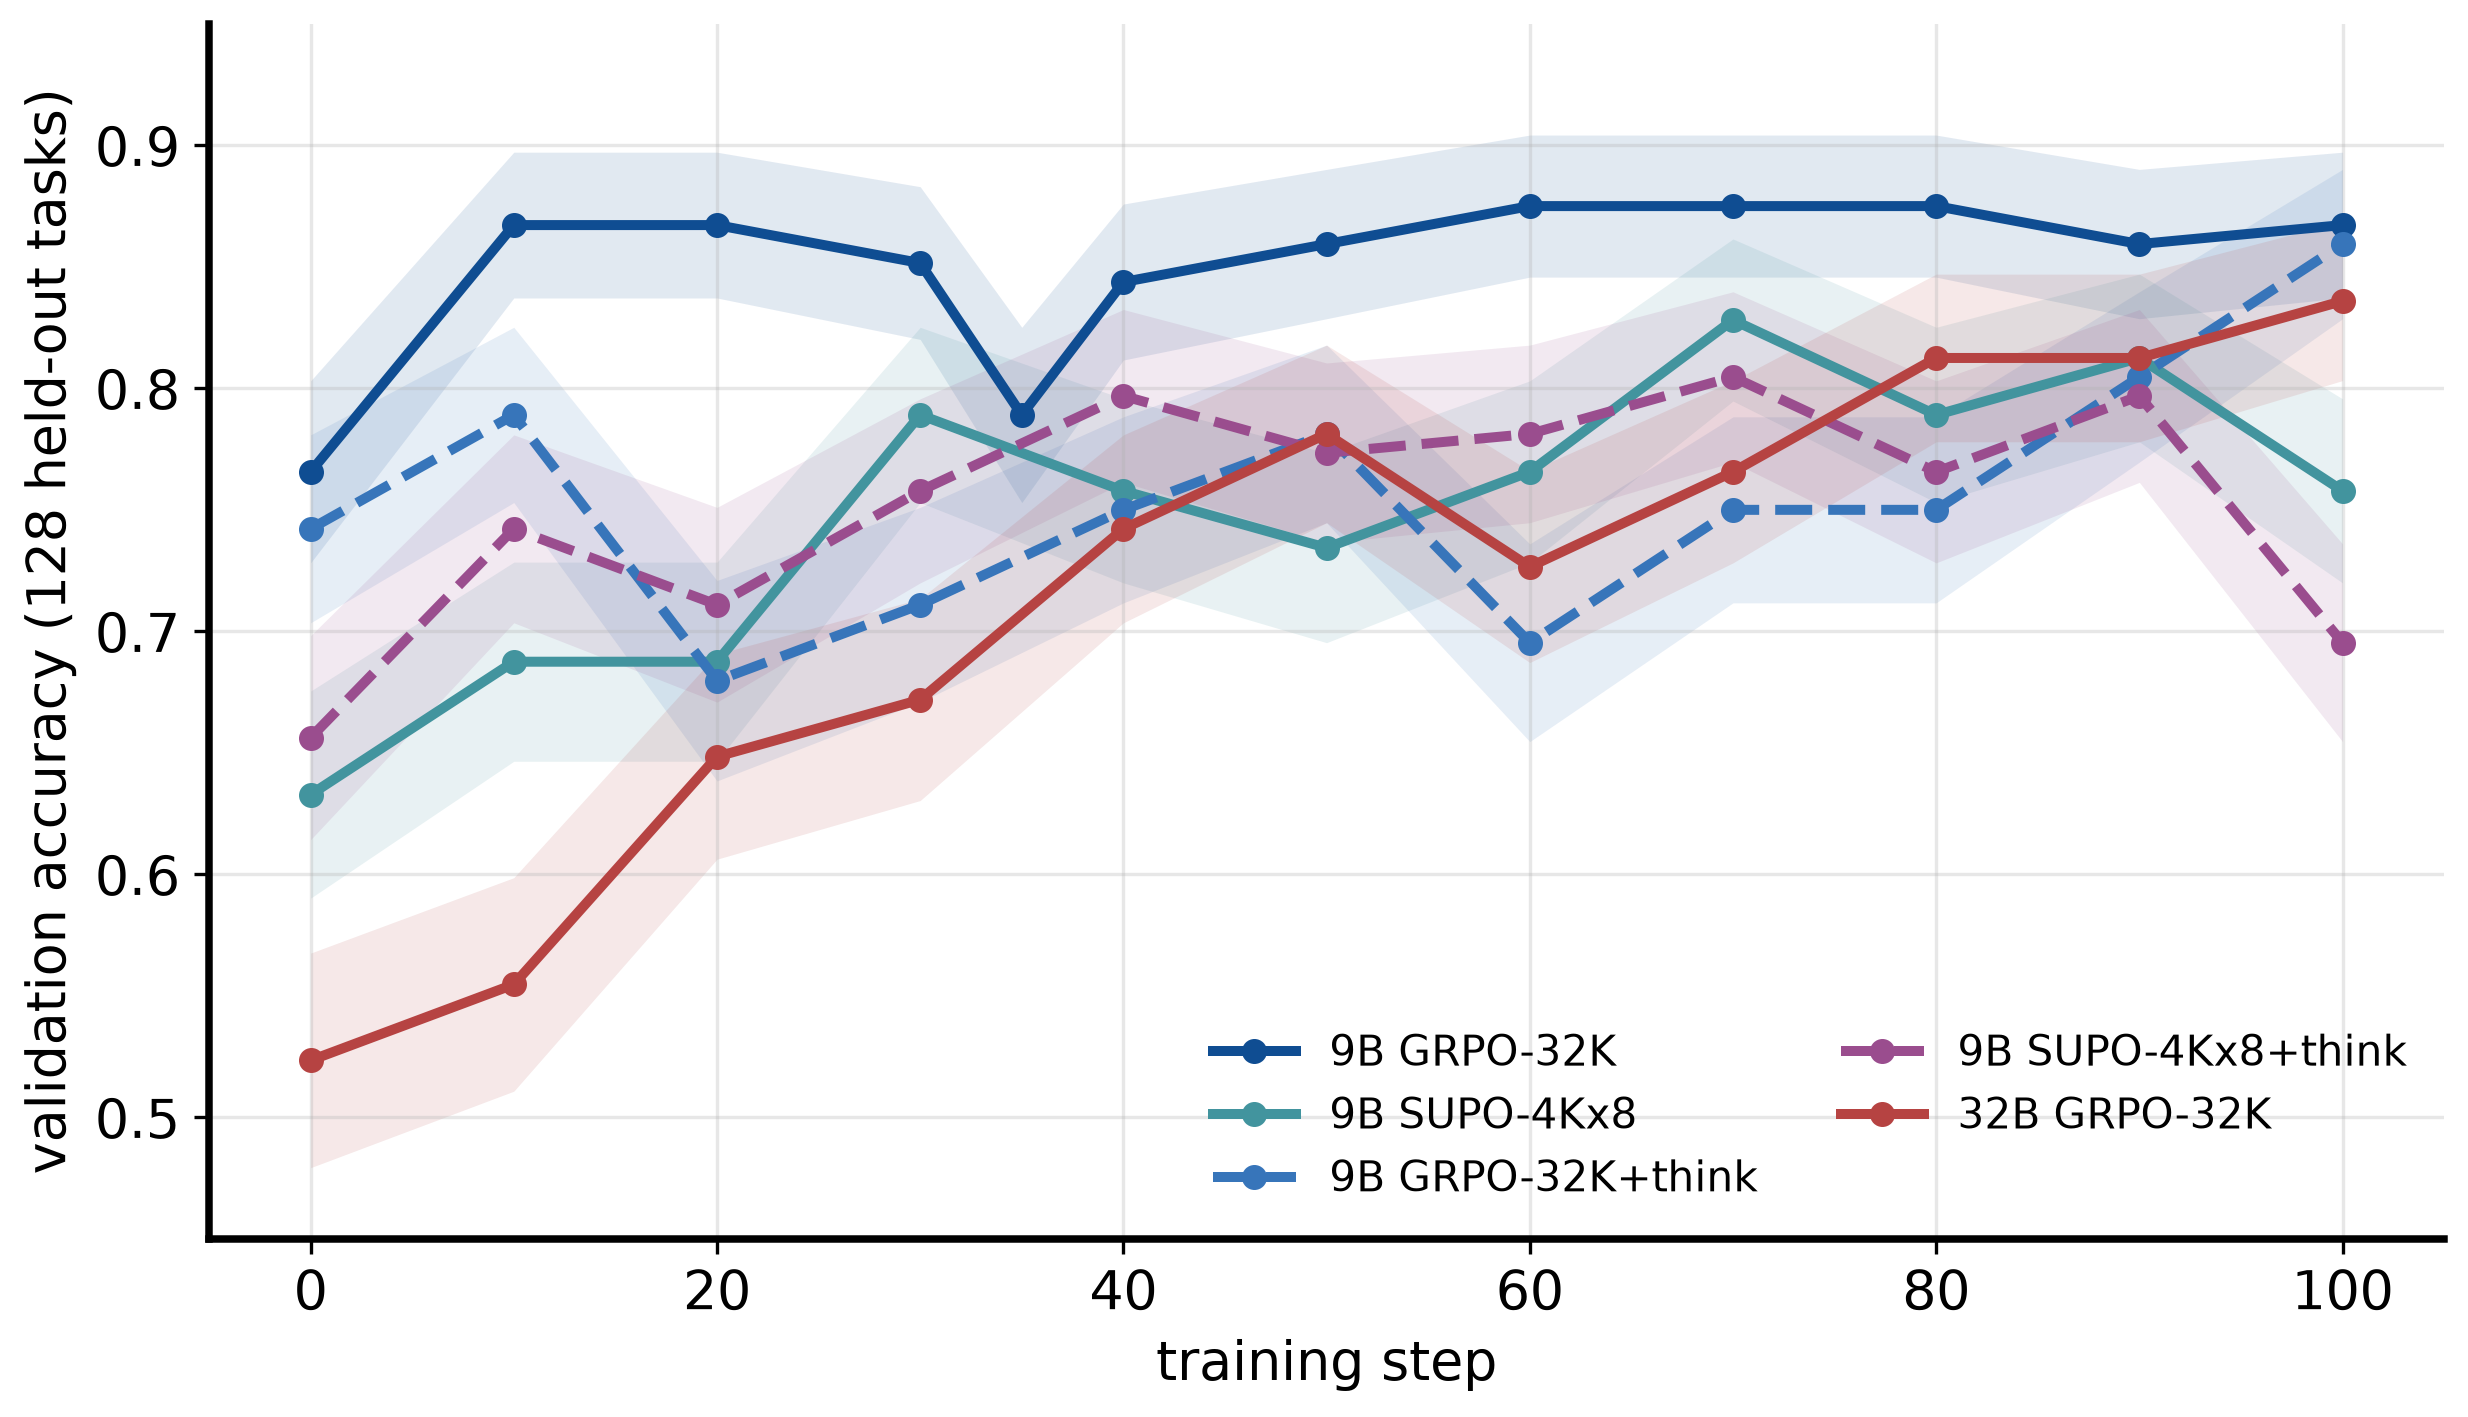
\includegraphics[width=0.9\textwidth]{fig1_val_acc_all_arms.png}
\caption{Greedy validation accuracy on the 128 held-out CodeGym tasks after every 10 training steps, for the two base-report arms (solid, blue/teal), their thinking variants (dashed) and the Qwen2.5-32B-Instruct GRPO arm (red). Shaded bands are $\pm1$ standard error $\sqrt{p(1-p)/128}$. Each point is the mean of the binary \p{score} field over the 128 records of \p{outputs/<exp>/val/<step>.jsonl}. Thinking hurts GRPO for most of the run and only catches up at step 100; thinking never helps SUPO; the 32B model starts 0.24 below the 9B model and closes most of the gap by step 80. Data: \p{fig1\_val\_acc\_all\_arms.csv}.}
\label{fig:val}\end{figure}

\begin{table}[h]\centering\small
\caption{Validation accuracy per checkpoint (greedy, $n=128$). ``final'' is step 100, ``peak'' the best checkpoint, ``mean 80--100'' the mean of the last three checkpoints. Source: \p{tables.md} / \p{val\_metrics.csv}.}
\label{tab:val}
\setlength{\tabcolsep}{3pt}\footnotesize
\begin{tabular}{@{}lccccccccccc|ccc@{}}\toprule
arm & 0 & 10 & 20 & 30 & 40 & 50 & 60 & 70 & 80 & 90 & 100 & final & peak & 80--100\\ \midrule
9B GRPO-32K & .766 & .867 & .867 & .852 & .844 & .859 & .875 & .875 & .875 & .859 & .867 & \textbf{.867} & .875 @60 & .867\\
9B SUPO-4K$\times$8 & .633 & .688 & .688 & .789 & .758 & .734 & .766 & .828 & .789 & .812 & .758 & \textbf{.758} & .828 @70 & .786\\
9B GRPO-32K+think & .742 & .789 & .680 & .711 & .750 & .781 & .695 & .750 & .750 & .805 & .859 & \textbf{.859} & .859 @100 & .805\\
9B SUPO-4K$\times$8+think & .656 & .742 & .711 & .758 & .797 & .773 & .781 & .805 & .766 & .797 & .695 & \textbf{.695} & .805 @70 & .753\\
32B GRPO-32K & .523 & .555 & .648 & .672 & .742 & .781 & .727 & .766 & .812 & .812 & .836 & \textbf{.836} & .836 @100 & .820\\
\bottomrule\end{tabular}
\end{table}

\paragraph{Thinking verdict.} On the same tasks and step budget, enabling thinking changes the final accuracy by $-0.008$ for GRPO-32K (0.867 $\to$ 0.859; within noise) and by $-0.063$ for SUPO-4K$\times$8 (0.758 $\to$ 0.695; peaks 0.828 vs.\ 0.805). Averaged over the last three checkpoints, which is the more robust summary, thinking costs 0.062 for GRPO (0.867 $\to$ 0.805) and 0.033 for SUPO (0.786 $\to$ 0.753). The thinking arms also cost more compute: median step time 946~s vs.\ 794~s for GRPO (Table~\ref{tab:beh}).

\paragraph{32B vs.\ 9B.} Qwen2.5-32B-Instruct starts at 0.523 and ends at 0.836 ($+0.312$), Qwen3.5-9B at 0.766 and 0.867 ($+0.102$). The 32B curve is still rising at step 100 (0.812, 0.812, 0.836 over the last three checkpoints) whereas the 9B curve is flat from step 10 on.

\subsection{Behaviour: truncation, tool calls, thinking length}
\begin{figure}[h]\centering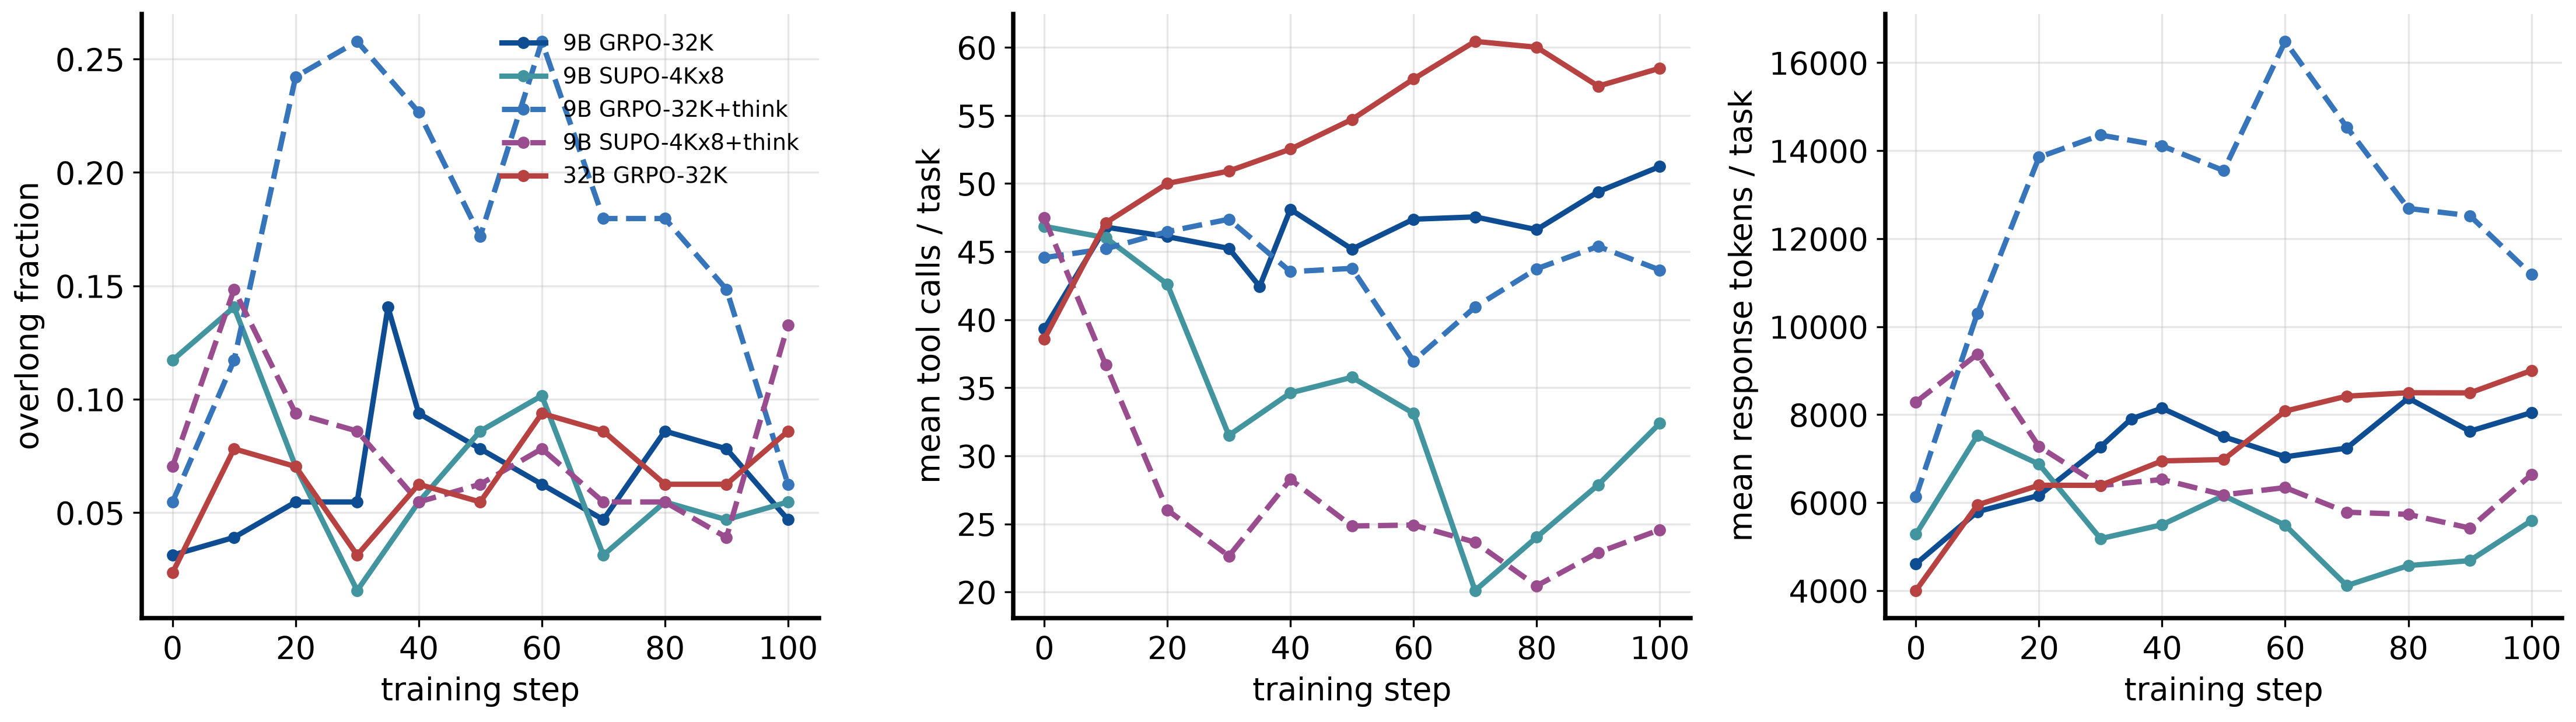
\includegraphics[width=\textwidth]{fig2_overlong_calls_tokens.png}
\caption{Per-checkpoint behaviour on the validation set (mean over the 128 episodes). Left: fraction of episodes flagged \p{overlong} (the episode hit the 100-call limit, the working-context limit, or ten consecutive turns without a function call). Middle: mean number of tool calls per episode. Right: mean generated tokens per episode (\p{rollout\_response\_tokens}, thinking included). GRPO+think truncates 15--26\% of episodes between steps 20 and 90 while generating $\sim$11K tokens per episode; the non-thinking GRPO arm stays at 3--9\% and $\sim$8K. SUPO+think keeps truncation low (4--9\%) except at step 100 (13\%) and makes the fewest tool calls (24.6 at step 100). Data: \p{fig2\_overlong\_calls\_tokens.csv}.}
\label{fig:beh}\end{figure}

\begin{table}[h]\centering\small
\caption{Behaviour at the first and last checkpoint and training cost. Overlong and tool calls from the validation dumps; the median step time is \p{timing\_s/step} over the logged steps of each arm's trainer log (see the deviations list for the two resumed logs). Source: \p{summary.json}.}
\label{tab:beh}
\setlength{\tabcolsep}{4pt}\footnotesize
\begin{tabular}{@{}lcccccc@{}}\toprule
arm & overlong @0 & overlong @100 & tool calls @0 & tool calls @100 & summaries @100 & median step (s)\\ \midrule
9B GRPO-32K & 0.03 & 0.05 & 39.3 & 51.2 & 0.00 & 794\\
9B SUPO-4K$\times$8 & 0.12 & 0.05 & 46.9 & 32.4 & 1.32 & 539\\
9B GRPO-32K+think & 0.05 & 0.06 & 44.6 & 43.6 & 0.00 & 946\\
9B SUPO-4K$\times$8+think & 0.07 & 0.13 & 47.5 & 24.6 & 1.98 & 551\\
32B GRPO-32K & 0.02 & 0.09 & 38.6 & 58.5 & 0.00 & 639 (16 GPUs)\\
\bottomrule\end{tabular}
\end{table}

\begin{figure}[h]\centering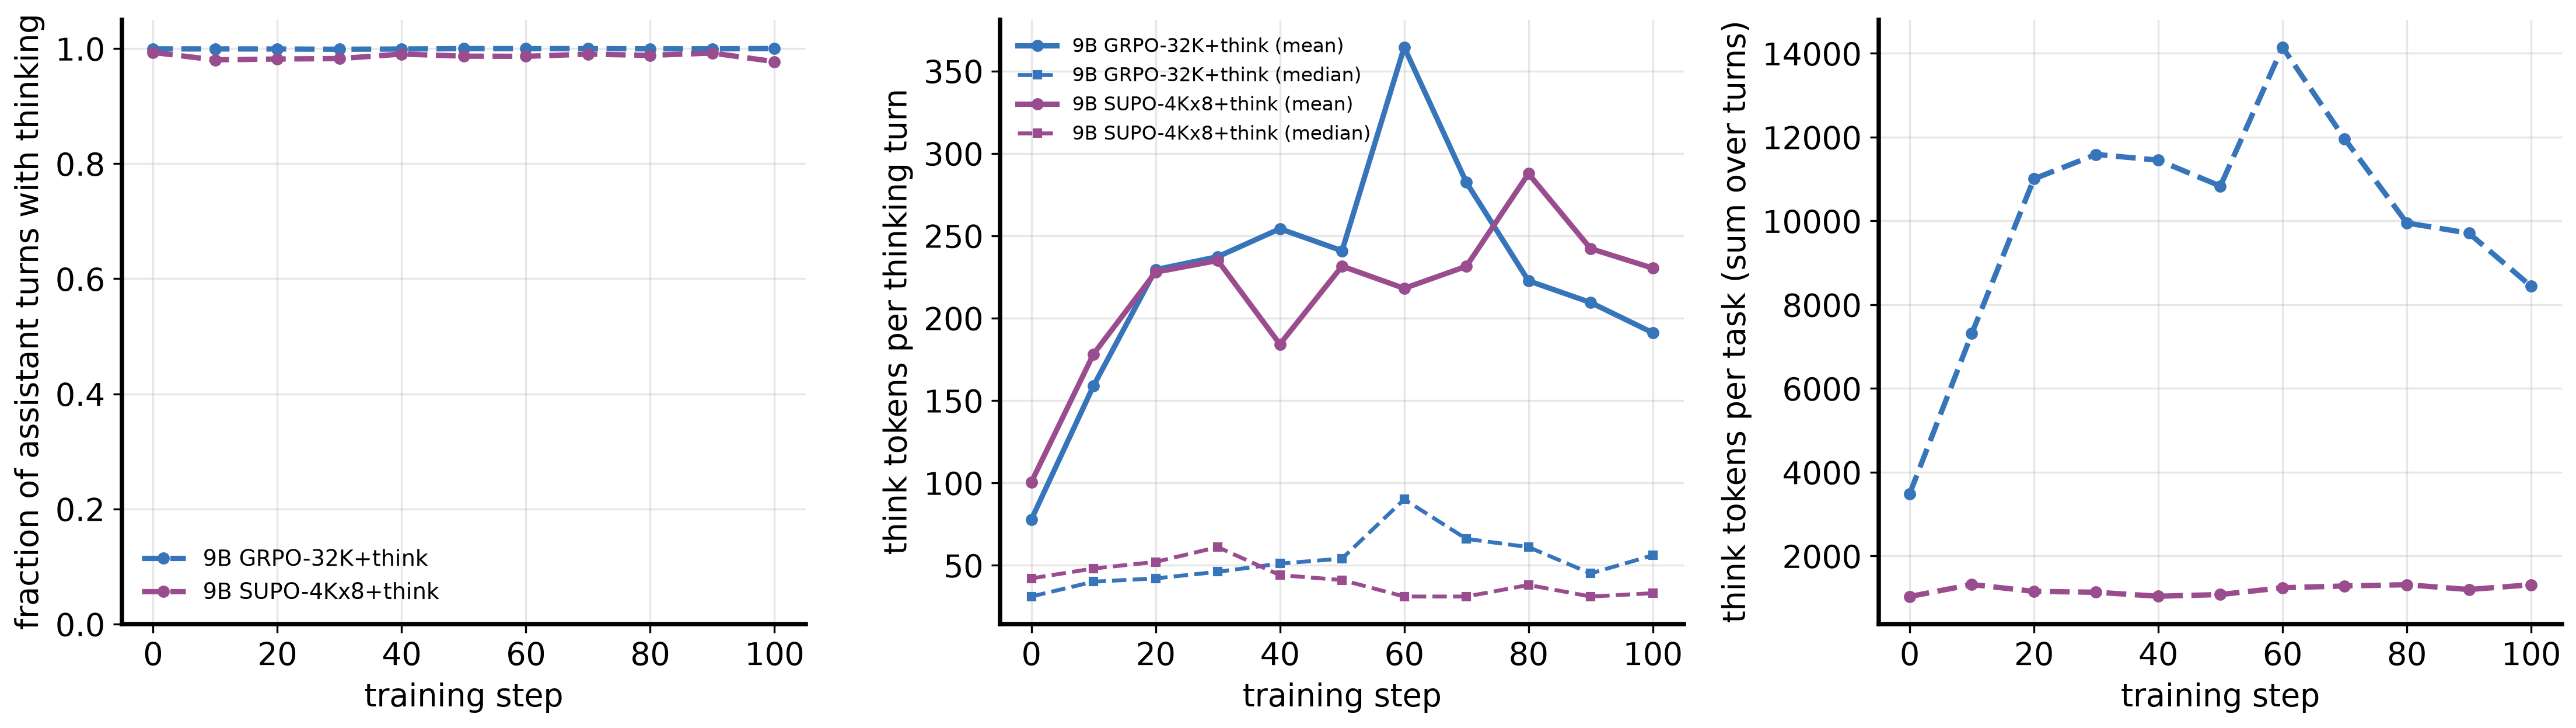
\includegraphics[width=\textwidth]{fig3_thinking_stats.png}
\caption{Thinking statistics of the two thinking arms per checkpoint, measured on the greedy validation outputs (\p{output} field of the validation dumps: the decoded generation including the chat-template role text). Each assistant turn is obtained by splitting on the template's \p{assistant} marker; a turn counts as a thinking turn when the text before its \p{</think>} tag (opening tag removed; for the first turn the template supplies the opening tag inside the prompt) is non-empty, or when a \p{<think>} block is opened but never closed (the turn was cut by the 4{,}096-token per-turn cap). Think tokens are counted with the Qwen3.5-9B tokenizer. Left: fraction of turns with thinking (99--100\% for GRPO+think, 96--99\% for SUPO+think; the non-thinking control arms measure exactly 0). Middle: mean (solid) and median (dashed) think tokens per thinking turn; the median stays at 30--60 tokens while the mean grows from 78 (step 0) to 240--360 (steps 40--60) and back to 190 (step 100) for GRPO+think, i.e.\ a heavy tail of very long thoughts (p90 up to 610 tokens, maximum 4{,}140 = the cap). Right: total think tokens per validation episode; GRPO+think spends 3.5K tokens per episode on thinking at step 0 and 8--14K in the middle of the run. Limitation: for SUPO the \p{output} field holds only the final working-context segment of each episode (600--1{,}300 turns per 128 tasks instead of $\sim$5{,}000), so its per-episode totals cover that segment only. Data: \p{fig3\_thinking\_stats.csv}.}
\label{fig:think}\end{figure}

The mechanism behind the GRPO+think dip is visible across Figures~\ref{fig:beh}--\ref{fig:think}: the policy's thinking grows from step 10 on, the per-episode generation grows to $\sim$11K tokens, more episodes overrun the 32K window and are masked out of the loss, and validation accuracy falls to 0.68--0.75. Between steps 60 and 100 the mean think length shrinks again (361 $\to$ 191 tokens per thinking turn), truncation falls from 26\% to 6\%, and accuracy recovers to 0.859. SUPO absorbs the extra thinking tokens through summarization, so its truncation stays low, but its thinking policy ends with fewer tool calls (24.6 vs.\ 32.4) and a lower final score.


\subsection{Thinking cut-offs by the per-turn cap}\label{sec:cutoff}
With \p{enable\_thinking} the Qwen3.5 generation prompt ends in \p{<think>\textbackslash n}, so every assistant turn starts inside a think block; a turn whose thinking never closed is one with no \p{</think>}. Per episode, \p{cut\_off\_turns = num\_steps - output.count("</think>")} (clipped at 0), computed by the builder from the greedy validation dumps of the GRPO-32K+think arm. Table~\ref{tab:cutoff} and Figure~\ref{fig:cutoff} report, per checkpoint, the cut-off turns over all turns, the fraction of episodes with at least one cut-off, the overlong rate and accuracy conditioned on whether the episode has a cut-off, and the mean response tokens per turn (\p{rollout\_response\_tokens / num\_steps}).

\begin{table}[h]\centering\footnotesize
\caption{Thinking cut-offs by the 4{,}096-token per-turn cap, 9B GRPO-32K+think, greedy validation ($n=128$ episodes per checkpoint). ``$\mid$ cut-off'' / ``$\mid$ none'' condition on the episode having $\ge 1$ / 0 cut-off turns. Source: \p{fig7\_think\_cutoffs.csv}.}
\label{tab:cutoff}
\setlength{\tabcolsep}{4pt}
\begin{tabular}{@{}rccccccc@{}}\toprule
step & cut-off / all turns & episodes w/ cut-off & overlong $\mid$ cut-off & overlong $\mid$ none & acc $\mid$ cut-off & acc $\mid$ none & tokens / turn\\ \midrule
0 & 24/5736 (0.4\%) & 6/128 (5\%) & 0.50 & 0.03 & 0.33 & 0.76 & 178\\
10 & 90/5888 (1.5\%) & 23/128 (18\%) & 0.52 & 0.03 & 0.39 & 0.88 & 300\\
20 & 188/6139 (3.1\%) & 39/128 (30\%) & 0.67 & 0.06 & 0.18 & 0.90 & 484\\
30 & 187/6251 (3.0\%) & 45/128 (35\%) & 0.62 & 0.06 & 0.36 & 0.90 & 504\\
40 & 193/5765 (3.3\%) & 41/128 (32\%) & 0.61 & 0.05 & 0.39 & 0.92 & 589\\
50 & 154/5756 (2.7\%) & 41/128 (32\%) & 0.51 & 0.01 & 0.46 & 0.93 & 509\\
60 & 236/4969 (4.7\%) & 50/128 (39\%) & 0.66 & 0.00 & 0.32 & 0.94 & 807\\
70 & 179/5420 (3.3\%) & 44/128 (34\%) & 0.52 & 0.00 & 0.34 & 0.96 & 586\\
80 & 129/5721 (2.3\%) & 37/128 (29\%) & 0.49 & 0.05 & 0.43 & 0.88 & 431\\
90 & 119/5931 (2.0\%) & 34/128 (27\%) & 0.50 & 0.02 & 0.44 & 0.94 & 461\\
100 & 62/5652 (1.1\%) & 33/128 (26\%) & 0.24 & 0.00 & 0.64 & 0.94 & 308\\
\bottomrule\end{tabular}
\end{table}

\begin{figure}[h]\centering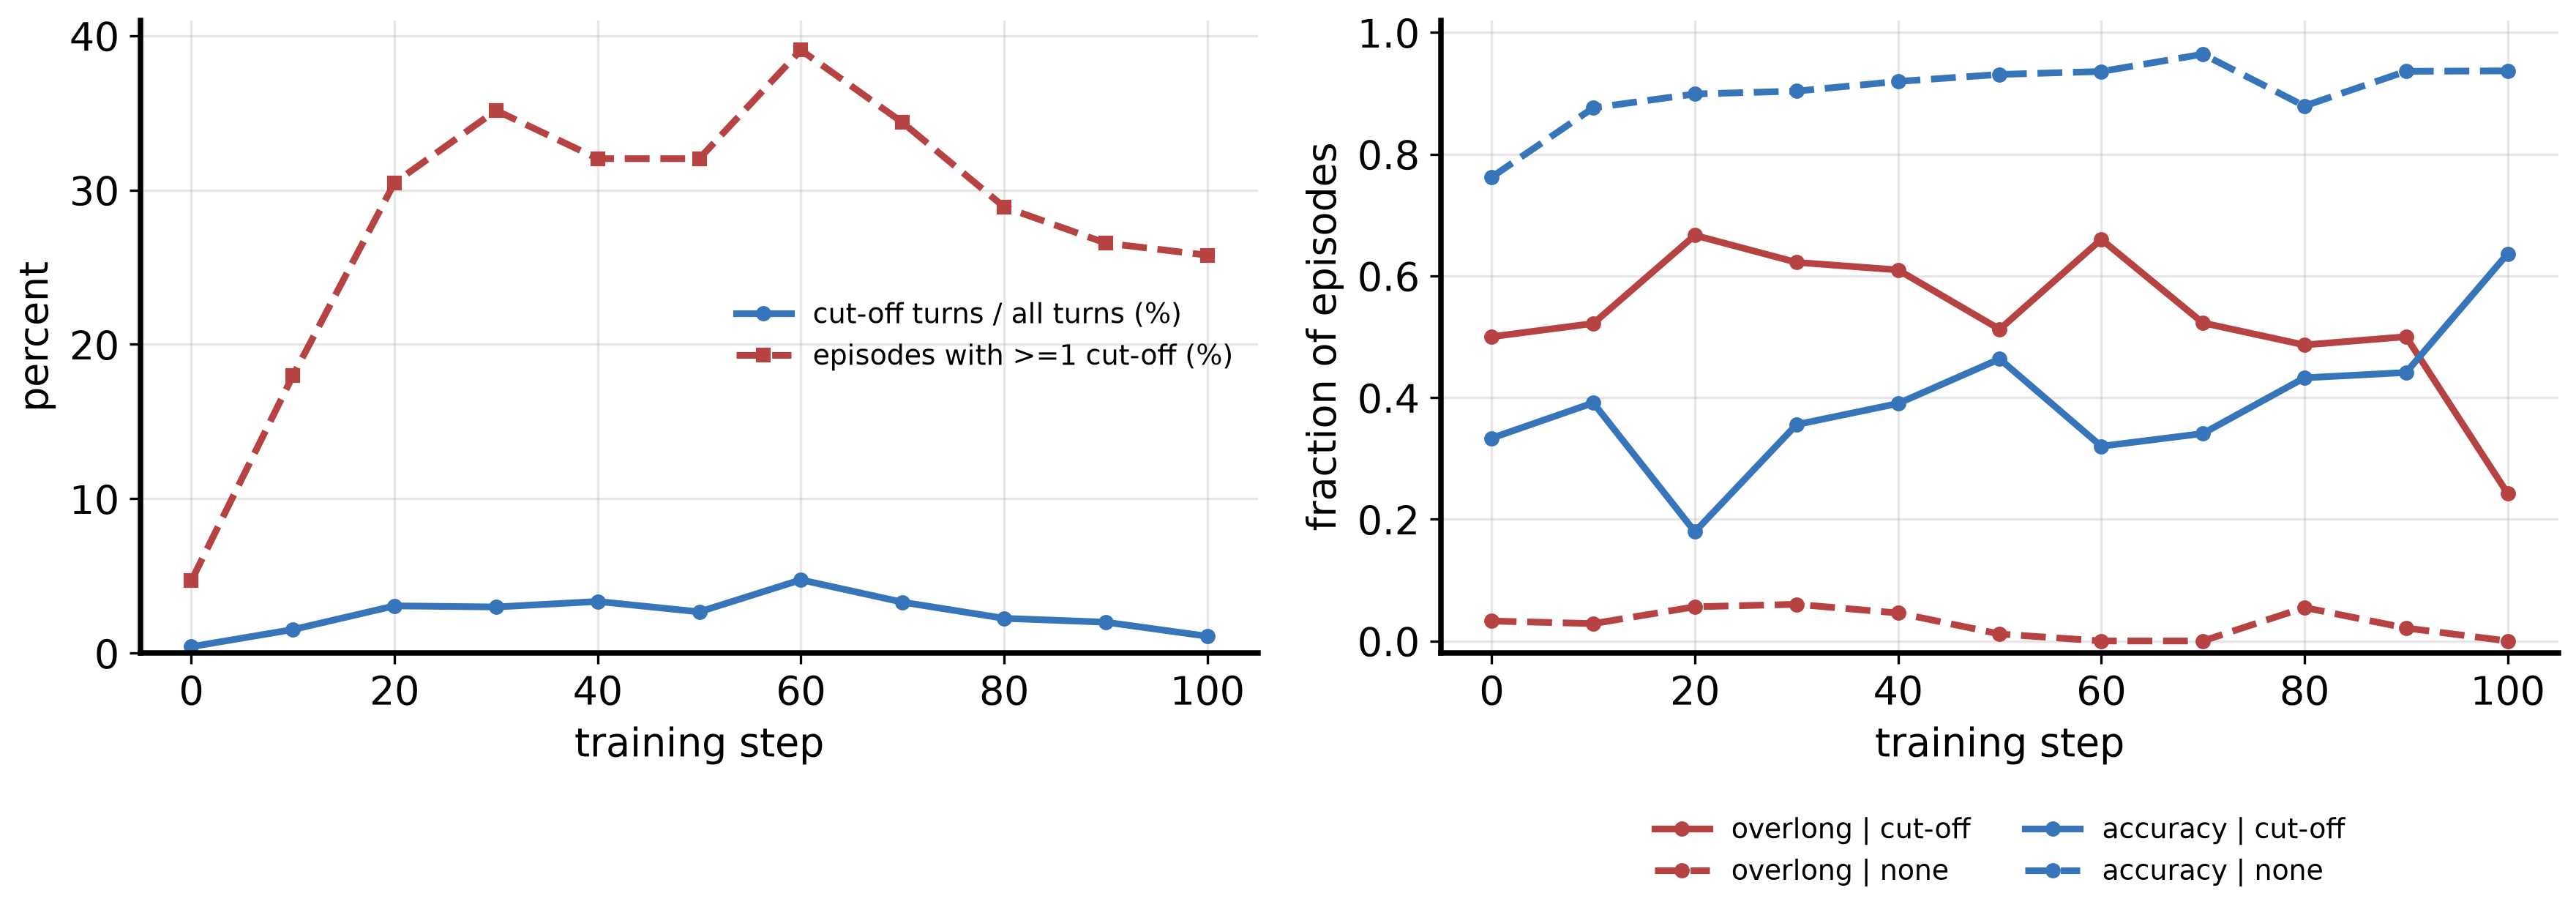
\includegraphics[width=\textwidth]{fig7_think_cutoffs.png}
\caption{Thinking cut-offs by the per-turn cap for 9B GRPO-32K+think per checkpoint (greedy validation, $n=128$). Method: with \p{enable\_thinking} the generation prompt ends in \p{<think>\textbackslash n}, so every assistant turn starts inside a think block, and a turn whose thinking never closed has no \p{</think>}; per episode \p{cut\_off\_turns = num\_steps - output.count("</think>")} (clipped at 0). Left: cut-off turns over all turns (solid) and episodes with at least one cut-off (dashed), in percent. Right: overlong rate (red) and accuracy (blue) conditioned on the episode having a cut-off (solid) or none (dashed). Data: \p{fig7\_think\_cutoffs.csv}.}
\label{fig:cutoff}\end{figure}

Only a few percent of turns overrun the 4{,}096-token cap (0.4\% at step 0, 3.1\% at 20, 4.7\% at 60, 1.1\% at 100), but they concentrate in a third of the episodes (5\% $\to$ 30\% $\to$ 39\% $\to$ 26\%) and wreck them: each cut-off turn burns $\sim$4K of the 30{,}720-token response budget and yields no action, so episodes with a cut-off are overlong 50--67\% of the time against 0--6\% for the others, and score 0.18--0.46 against 0.88--0.96 (Table~\ref{tab:cutoff}). The cut-off rate tracks the thinking-length growth of Figure~\ref{fig:think} and the validation dip between steps 20 and 60, and its fall to 1.1\% by step 100 (with overlong $\mid$ cut-off down to 0.24) matches the recovery to 0.859.

\emph{Ruled out.} The Qwen chat template drops earlier turns' \p{<think>} blocks when a conversation is re-rendered (the ``prefix-unstable'' behaviour), which could in principle remove thinking from the context or the training targets. That does not apply here: verl's continuous-token builder appends only rendered deltas and every generation call is fed the raw accumulated token stream (\p{supo/agent\_loop.py} \p{\_generate} passes \p{prompt\_ids=traj.token\_ids}; \p{verl/utils/tokenizer/continuous\_token.py} \p{\_merge\_context\_token\_ids}), so earlier thinking stays in the rollout context and in the training targets.

\emph{Caveats.} The metric is not applicable to the non-thinking control (its empty \p{<think></think>} pair sits in the prompt, so the count trivially flags one turn per episode) nor to multi-segment SUPO episodes (the \p{output} field keeps only the final working-context segment). Single-segment SUPO+think episodes ($n=21$--48 per checkpoint, \p{summary.json}) show zero cut-offs: the 4K working context triggers a summary before a turn can reach the cap.

\subsection{Training curves}
\begin{figure}[h]\centering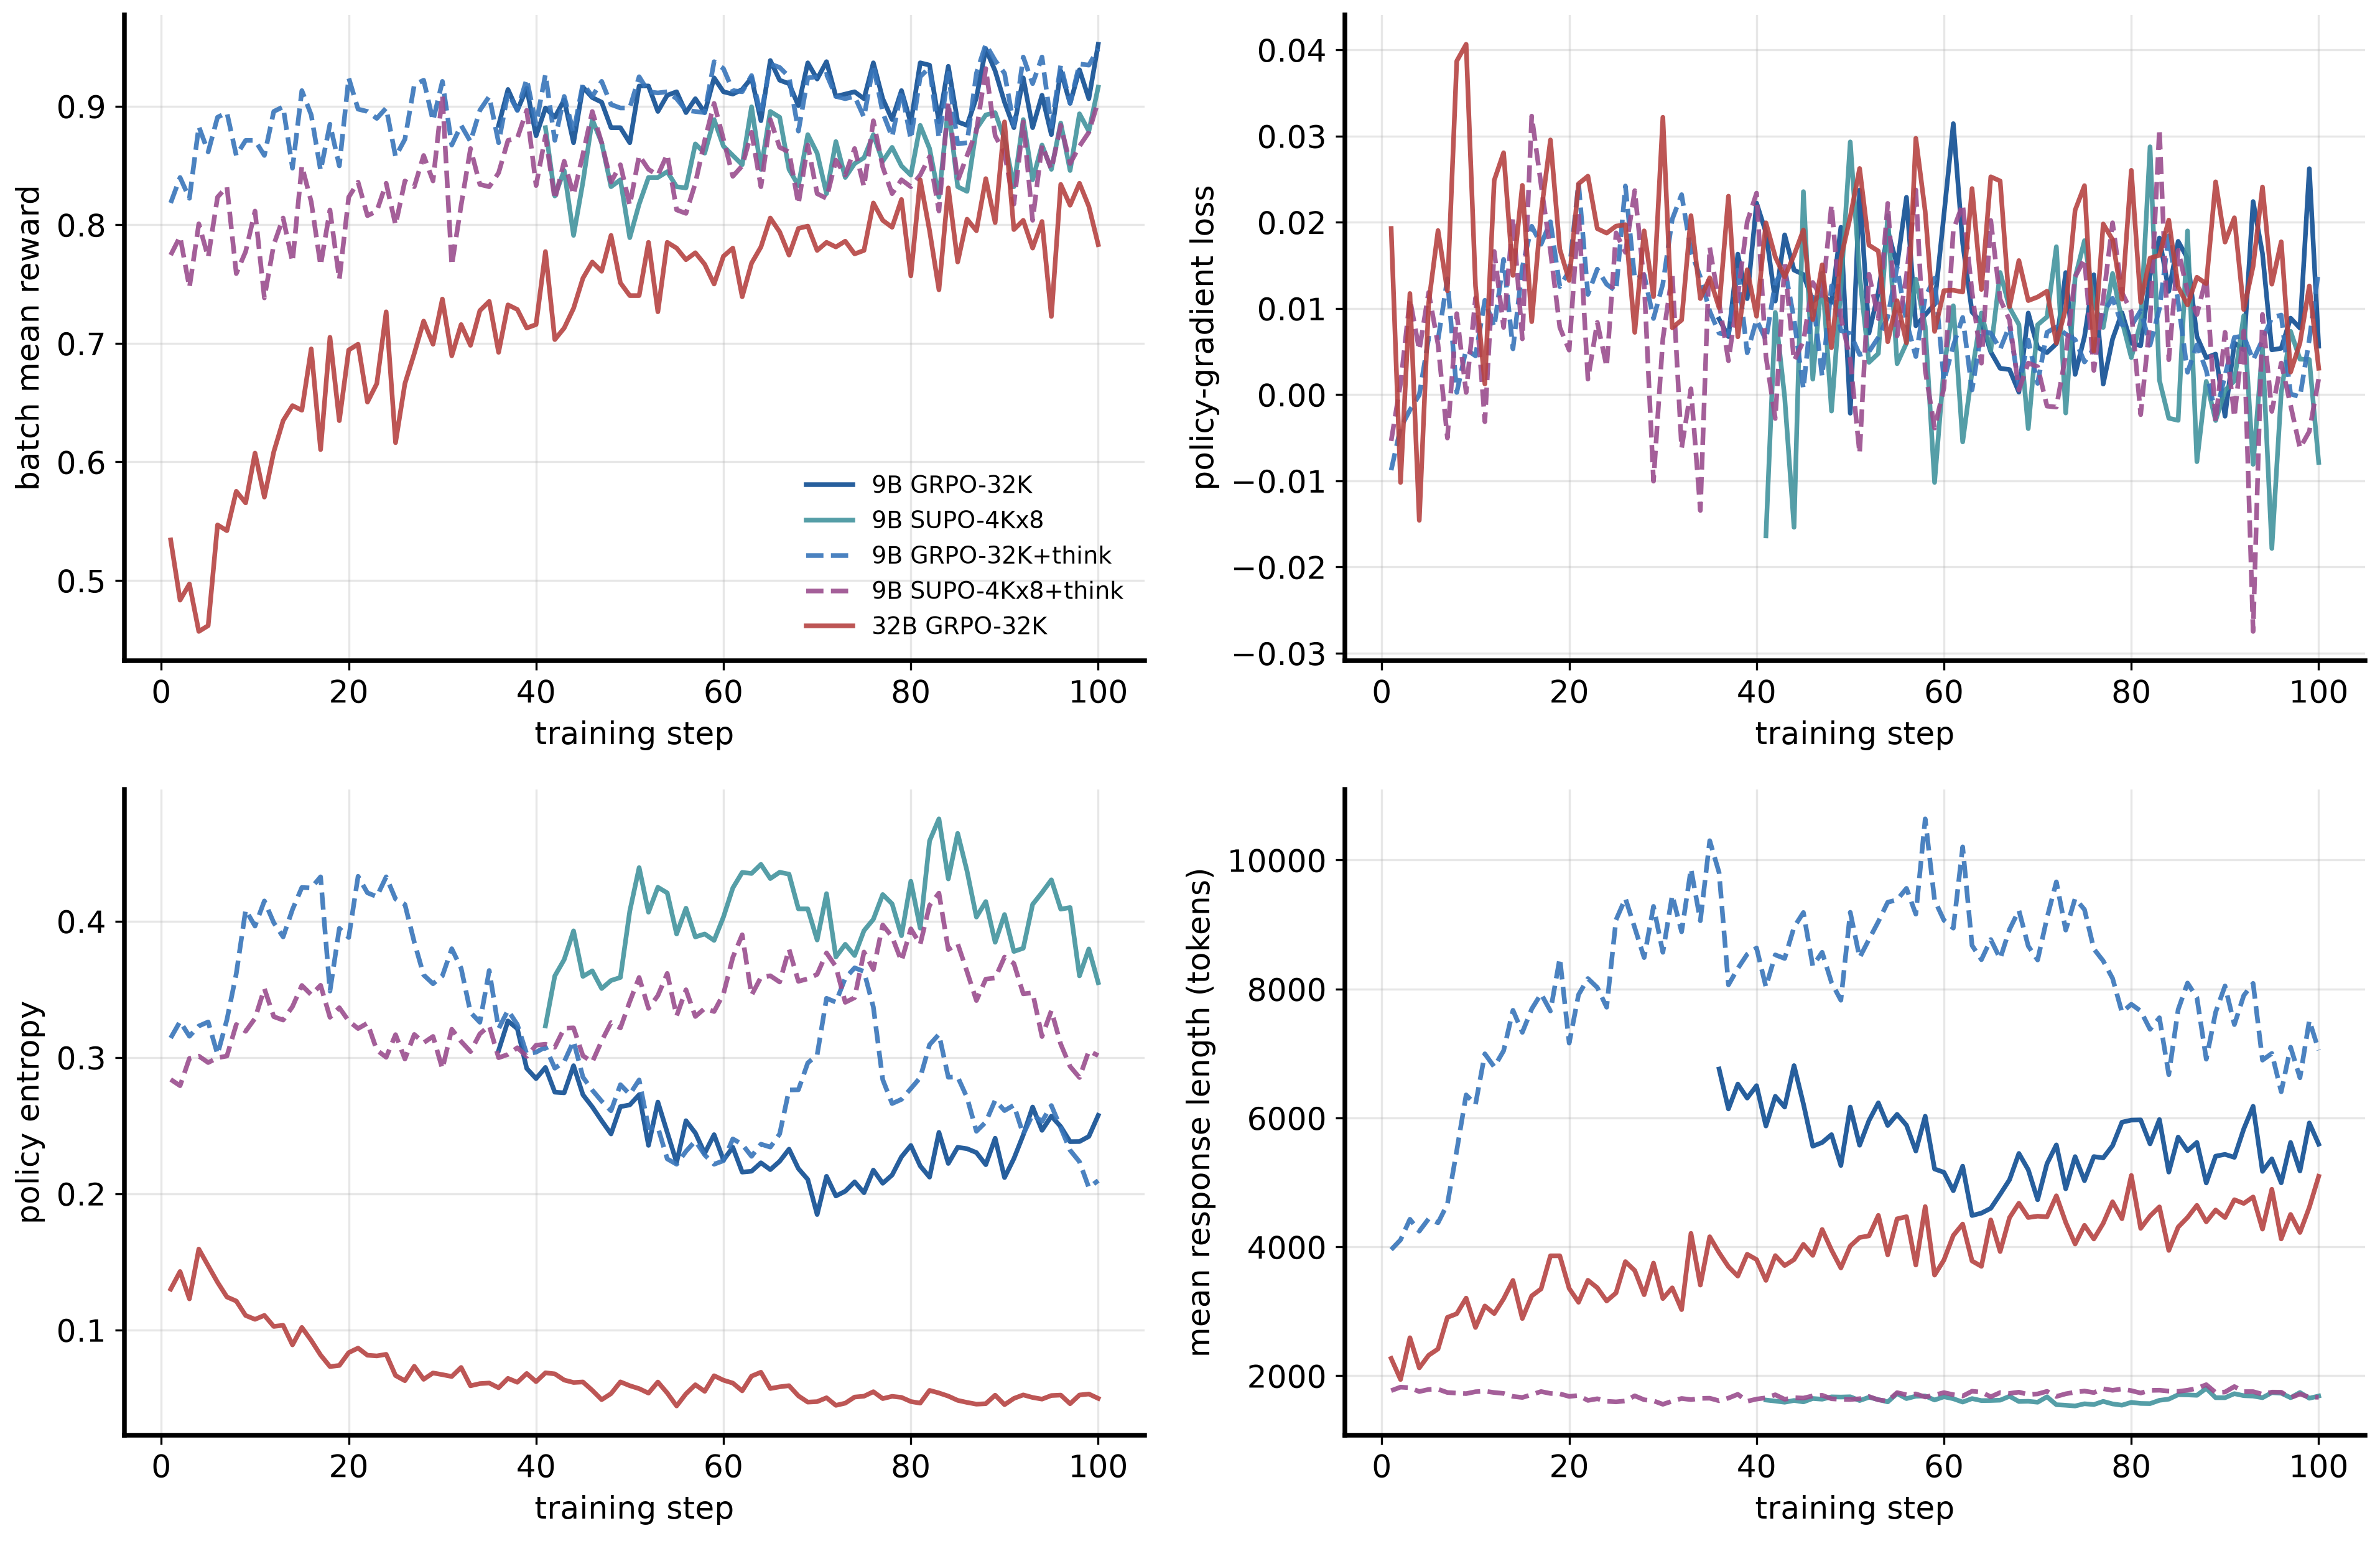
\includegraphics[width=\textwidth]{fig4_training_curves.png}
\caption{Batch-level trainer metrics parsed from the \p{step:N - key:value} lines of each arm's trainer stdout (ray and ANSI prefixes stripped, last occurrence per step kept). Top left: mean training reward of the batch (\p{critic/score/mean}, 128 prompts $\times$ 8 rollouts at temperature 1). Top right: policy-gradient loss. Bottom left: policy entropy (\p{actor/entropy}). Bottom right: mean generated tokens per rollout (\p{response\_length/mean}). The 9B non-thinking curves start at step 36/40 (resumed pods, see deviations). The 32B policy has a much lower entropy from the start (0.13 $\to$ 0.05) than the 9B policies (0.26--0.43) and its response length grows steadily (2.3K $\to$ 5.1K tokens) as it learns to make more calls per episode (38.6 $\to$ 58.5 on validation). GRPO+think produces the longest rollouts (up to 10.6K tokens at step 58) and its entropy rises during the dip and falls again as thinking shortens. Data: \p{fig4\_training\_curves.csv}.}
\label{fig:train}\end{figure}

\subsection{32B vs.\ 9B on the same tasks}
\begin{figure}[h]\centering
\begin{subfigure}[t]{0.58\textwidth}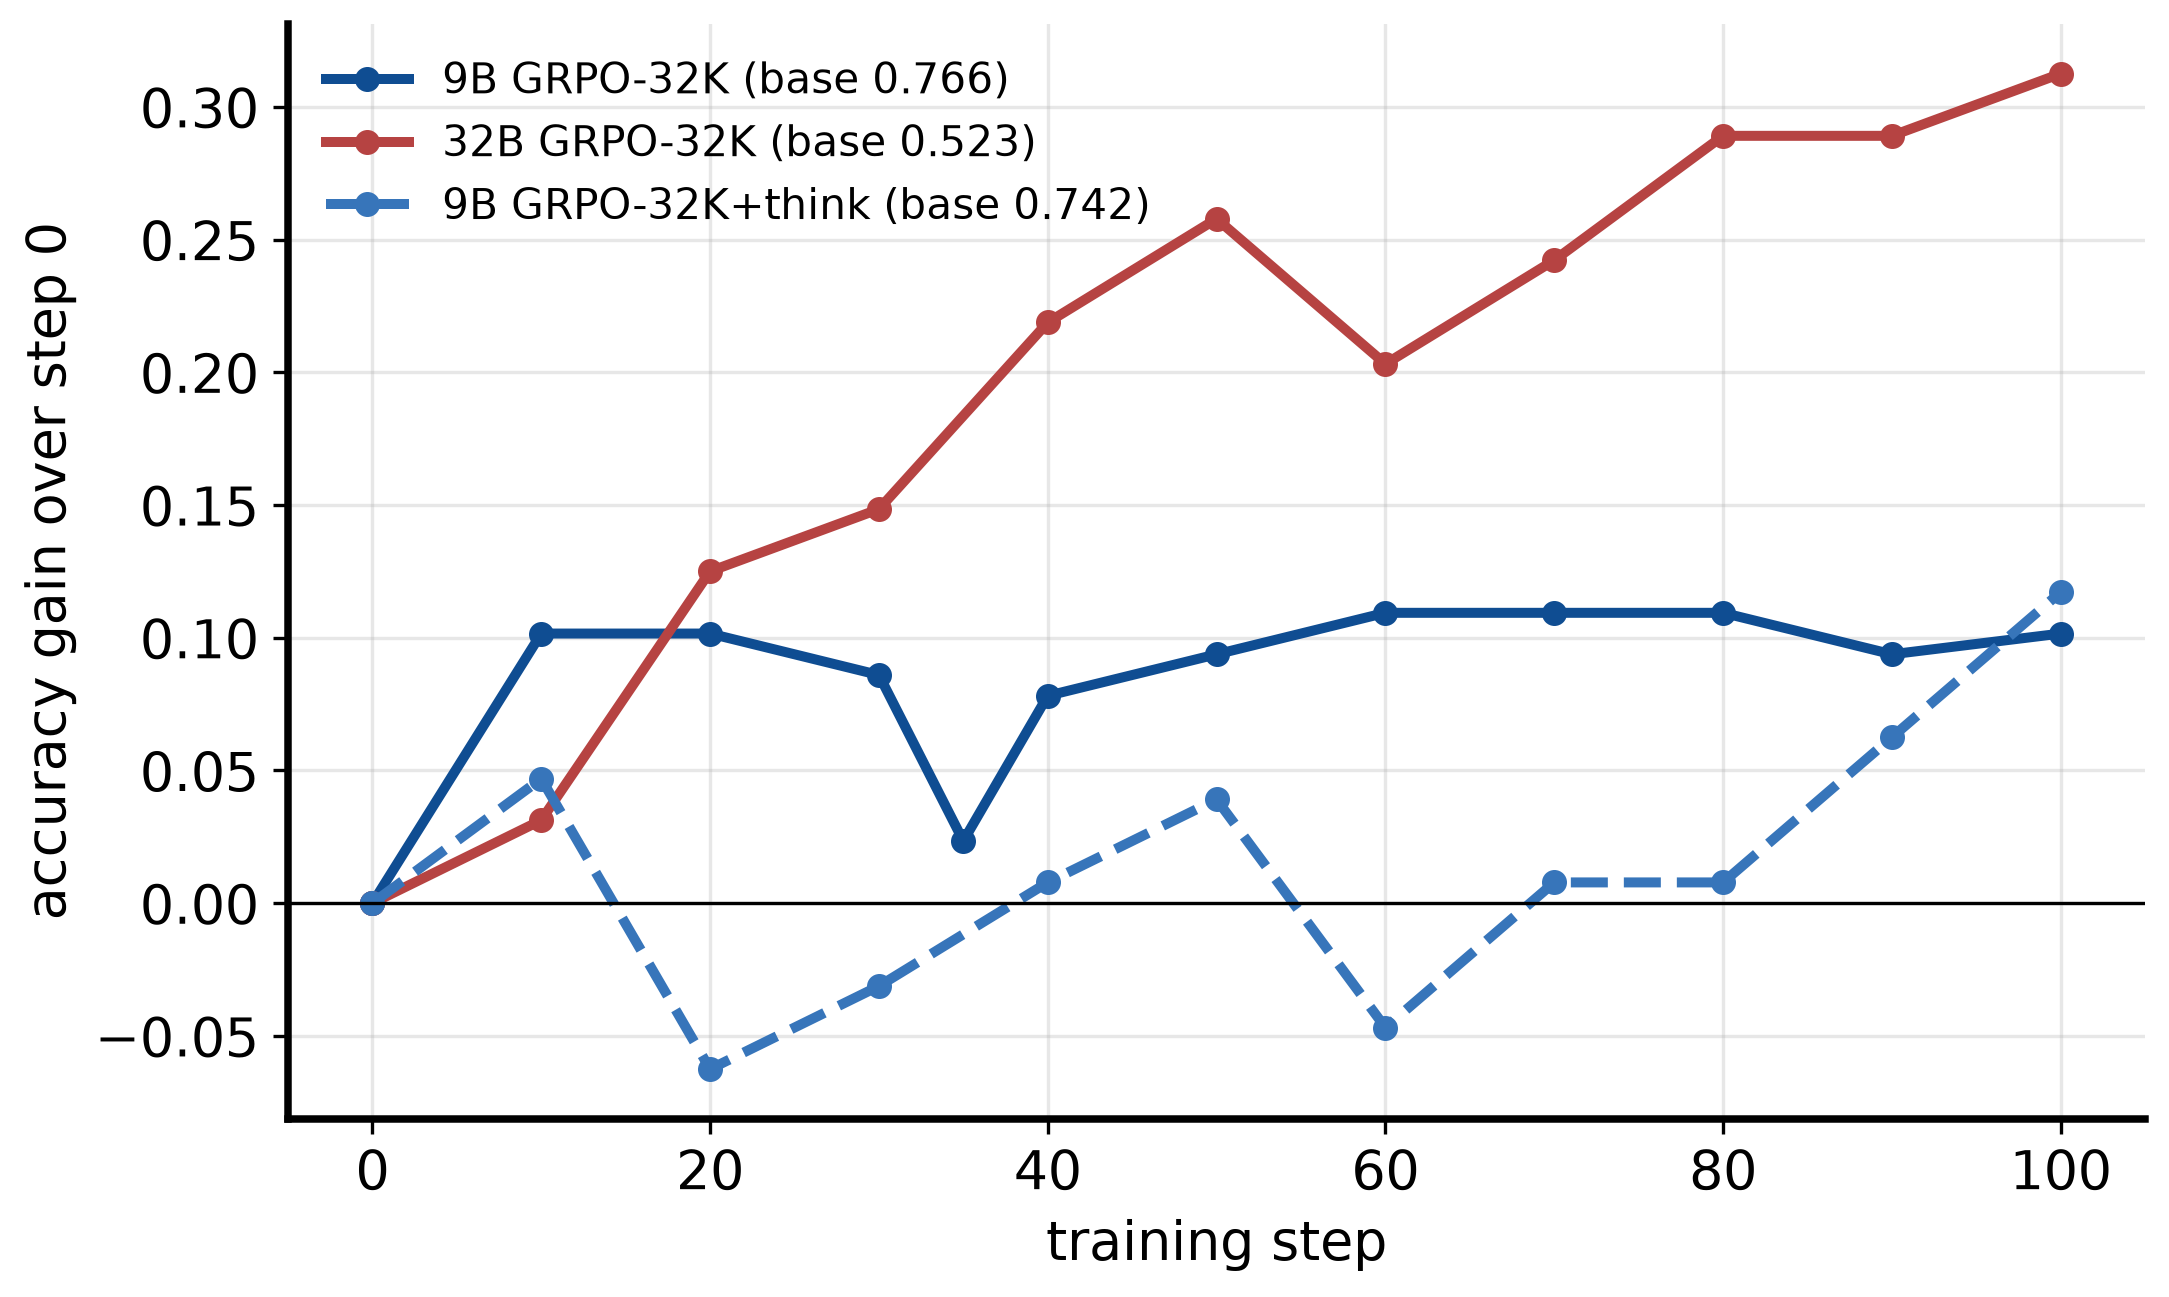
\includegraphics[width=\textwidth]{fig5_gain_over_base.png}\caption{Accuracy gain over the arm's own step-0 accuracy.}\end{subfigure}\hfill
\begin{subfigure}[t]{0.38\textwidth}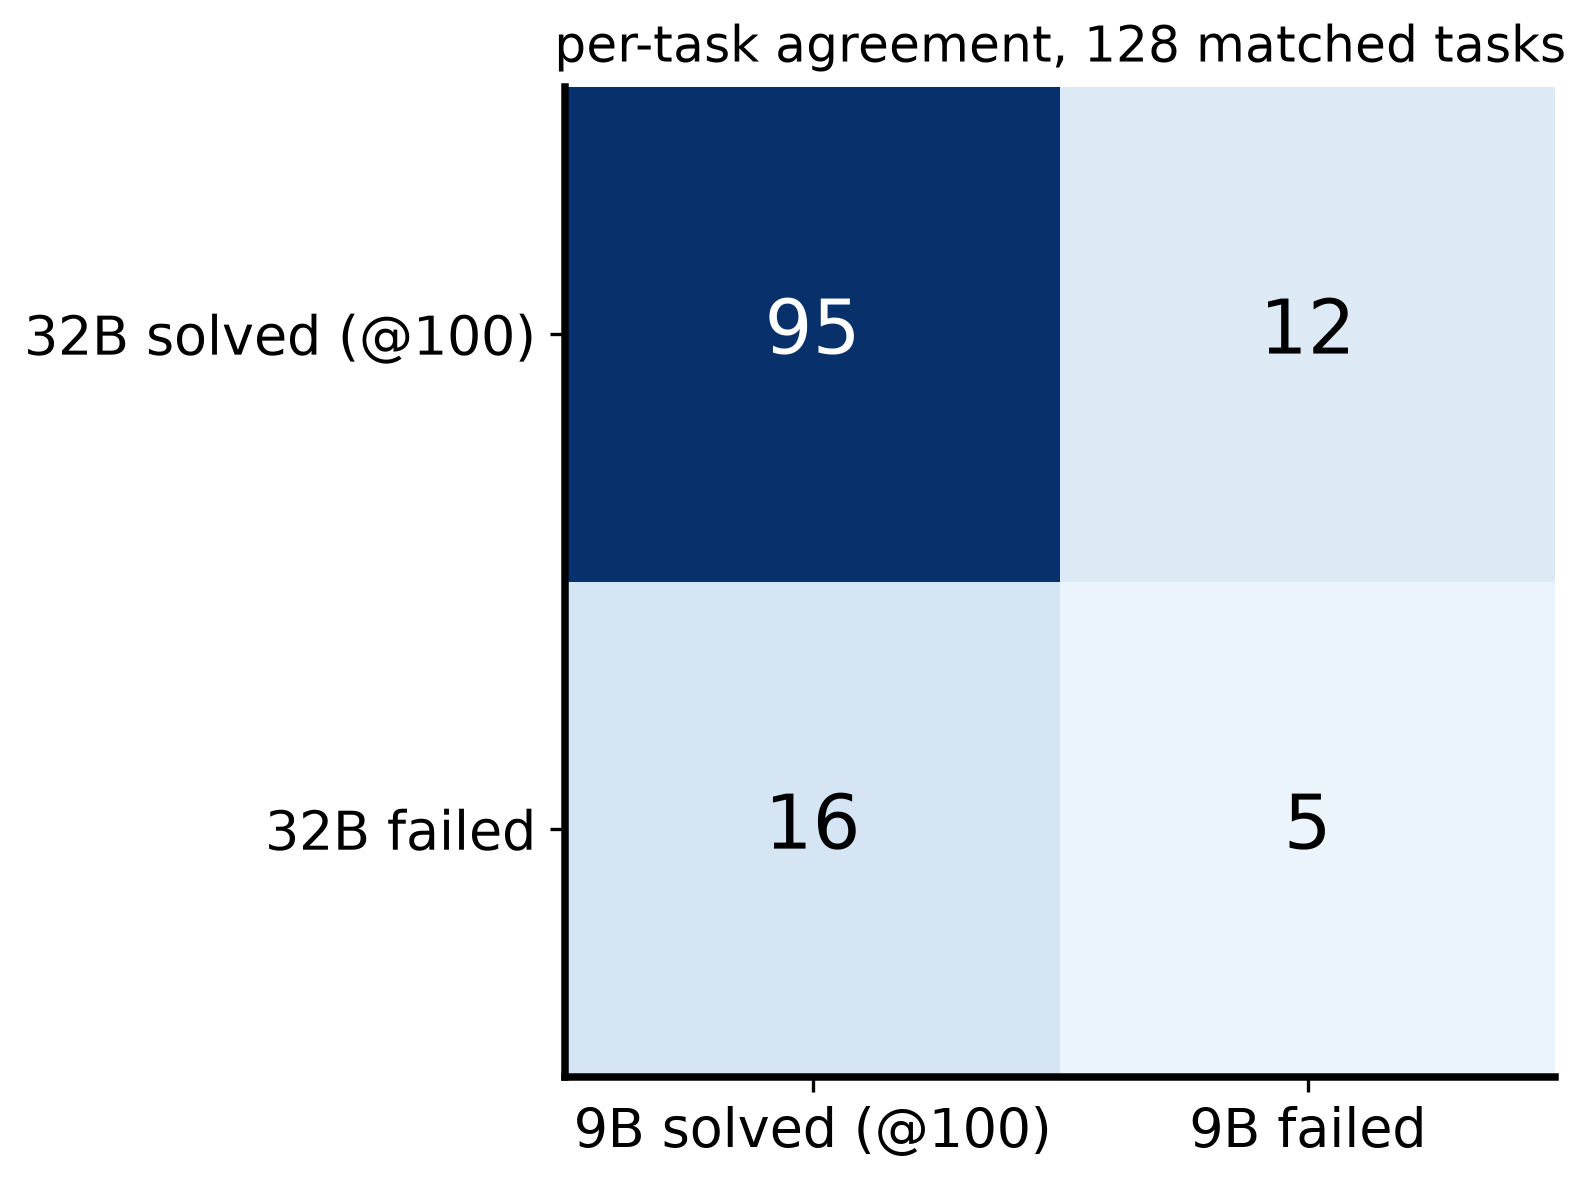
\includegraphics[width=\textwidth]{fig6_task_agreement.png}\caption{Per-task agreement at step 100.}\end{subfigure}
\caption{(a) Gain over base for the three GRPO-32K arms: the 32B model gains $+0.31$ against $+0.10$ for the 9B model, but from a base 0.24 lower. (b) Solved/unsolved contingency between the final 32B and 9B GRPO policies on the 128 tasks, matched across runs by an MD5 of the validation prompt text with chat-template role markers, thinking scaffolds and whitespace removed (128 of 128 matched). Both solve 95 tasks; 16 are solved only by the 9B policy, 12 only by the 32B policy, 5 by neither. Of the 30 tasks the 9B \emph{base} model failed at step 0, the final 9B policy solves 19 and the final 32B policy also solves 19. Data: \p{fig5\_gain\_over\_base.csv}, \p{fig6\_task\_agreement.json}.}
\label{fig:cmp}\end{figure}

\subsection{Comparison with the CodeGym paper}\label{sec:paper}
The CodeGym paper~\cite{codegym} reports, for Qwen2.5-32B-Instruct, an in-domain success rate of 30.1\% before RL and 81.0\% after (75.0\% without its data filters). Table~\ref{tab:paper} lists why those levels are not comparable with ours, although the direction and the size of the RL gain are.
\begin{table}[h]\centering\small
\caption{Evaluation protocol of the CodeGym paper (from its text) vs.\ this report.}
\label{tab:paper}
\begin{tabular}{@{}p{3.2cm}p{6.2cm}p{6.2cm}@{}}\toprule
 & CodeGym paper (arXiv 2509.17325) & this report\\ \midrule
evaluation set & 500 unseen environments, 972 task configurations & 128 unseen seed problems, 128 tasks\\
difficulty filter & 10--256 required tool calls \emph{and} base-model accuracy $\le 25\%$ & oracle solution 40--90 calls; no accuracy filter\\
decoding & temperature 0.7, top-p 0.95, pass@1 & greedy, one attempt\\
tool-call budget & 256 (512 for the hard variant) & 100\\
context & 5{,}120 prompt $+$ 24{,}576 response & 2{,}048 $+$ 30{,}720\\
training & GRPO, 512 prompts $\times$ 8, $\sim$100 steps & GRPO, 128 prompts $\times$ 8, 100 steps\\
Qwen2.5-32B-Instruct & 30.1 $\to$ 81.0 (filtered data) / 75.0 (unfiltered) & 0.523 $\to$ 0.836\\
\bottomrule\end{tabular}
\end{table}
The paper's $\le 25\%$ accuracy screen fixes the base score near the screening threshold by construction, and its 50-point gain is measured on tasks selected because the base model fails them. Our set never removes tasks the base model solves, so a strong model starts high; the 32B base at 0.52 (0.39--0.50 in earlier two-step smoke runs, $n=128$ each) is the same model on a less adversarial pool with greedy decoding. A direct number against the paper would require rebuilding an evaluation split with both of its filters and re-scoring the saved checkpoints (steps 80 and 100 of the 32B run and steps 95/100 of the 9B runs are on HDFS); that is a data-preparation change, not a retrain.

\section{Example trajectories}
Excerpts rendered by \p{pretty\_traj} in the builder script (tool outputs truncated, long runs of turns elided); the full excerpts are in \p{assets/traj\_*.txt} and the records in \p{trajectories.json}.

\paragraph{32B, step 0, failure (sampled training rollout).} The base model follows the protocol but merges the strings one character at a time and submits a wrong answer after 62 calls.
\lstinputlisting{assets/traj_32B_step0_failure.txt}

\paragraph{32B, step 100, success.} Same environment as the failure below (two rollouts of the same prompt in the step-100 batch). The policy recovers from a malformed first call, plans the full search, and submits the right answer after 79 calls.
\lstinputlisting{assets/traj_32B_step100_success.txt}

\paragraph{32B, step 100, failure.} The sibling rollout re-observes the grid after every reset, runs out of the 100-call budget (\p{stop=max\_steps}, overlong) and never submits.
\lstinputlisting{assets/traj_32B_step100_failure.txt}

\paragraph{9B GRPO-32K+think, step 100, validation episode with packed thinking.} First four turns of the first solved validation task; the first turn's think block is opened by the chat template and runs long, later turns think for a sentence or two before each call.
\lstinputlisting{assets/traj_9B_think_val_step_last.txt}

\section{Incident log and timeline (PDT)}
\begin{itemize}[nosep]
\item \textbf{Sep 8, 16:03} thinking arms launched (1$\times$8 H100 each); both ran uninterrupted to step 100 (SUPO+think done Sep 9 10:09, GRPO+think done Sep 9 20:31); both final checkpoints mirrored to HDFS.
\item \textbf{Sep 8, 19:00--Sep 9, 13:00} sixteen 2-node smoke runs (2 steps each) for the 32B arm, each exposing one defect: huggingface\_hub snapshot download hanging at $\sim$31~GB (replaced by per-file curl); \p{max\_model\_len} above the model's 32{,}768 positions; ray head start failing silently on the allocated port (port fallbacks, worker-port range pinned to 30000--39999); wandb ``No API key'' because ray daemons started before the env exports (\p{train\_env.sh} sourced first); a verl bug in \p{dense\_common}.\allowbreak\p{forward\_with\_triton\_backend} passing the fp32 lm-head weight with bf16 hidden states to the fused cross-entropy kernel (cast added, mirrored from the Qwen3.5 path); on A100 pods an InfiniBand GPU-Direct registration error (\p{NCCL\_NET\_GDR\_LEVEL}\allowbreak=\p{LOC}) and later a whole rack of IPv6-only pods (fail-fast preflight); a stale \p{DONE} marker in the shared run directory making the rank-1 pod leave the ray cluster at start (per-trial markers); verl's driver actor landing on rank 1 so that rank 0 never saw the checkpoint tracker file (mirror readiness now derived from each node's own shard files); HDFS-fuse dropping appends from a second writer (sync log made pod-local with a single-writer copy); and mawk printing the 196~GB byte sum in scientific notation, which aborted the upload in bash arithmetic (printf \%.0f).
\item \textbf{Sep 9, 10:47} the H100 smoke that had waited 13~h in the queue trained correctly on H100 (val 0.500/0.523/0.484 over two steps).
\item \textbf{Sep 9, 13:27} the queued smoke was converted into the full run at the user's request; pods after 92~min; trainer up at 15:06; 8--11~min per step.
\item \textbf{Sep 9, 18:34} first live checkpoint (step 20) mirrored from both nodes in 450~s (433--438~MB/s over the fuse fallback after the HDFS CLI puts failed fast with an empty error); steps 40/60/80/100 likewise (399--463~MB/s).
\item \textbf{Sep 10, 09:49} 32B run exited cleanly; checkpoints 80 and 100 complete on HDFS (two kept).
\end{itemize}
\paragraph{Open items.} The HDFS CLI put path fails immediately on the 32B pods (empty error text; the fuse fallback carried every upload, so low priority). The IPv6-only preflight may be stricter than needed now that the stale-marker bug, which produced the ``IPv6 hang'', is fixed. A paper-protocol evaluation split (call-count band plus base-accuracy screen) would enable a direct comparison with the CodeGym paper. Post-hoc evaluation of the saved checkpoints on that split is straightforward.

\section{Discussion and limitations}
\begin{itemize}[nosep]
\item \textbf{Training thinking at 32K needs a stop condition that closes thinking}: a think budget separate from the answer budget, or a larger per-turn cap with the overlong mask kept (Section~\ref{sec:cutoff}).
\item \textbf{Thinking is not free context.} With a fixed 32K window, a policy that thinks 3--14K tokens per episode leaves less room for tool calls and observations; GRPO's reward signal then pushes it to think less (Fig.~\ref{fig:think}), and only when it does does accuracy recover. SUPO's summaries hide the cost from the context but not from the policy: the thinking SUPO arm makes fewer calls and scores lower. On CodeGym, where the useful reasoning is a short plan followed by many cheap calls, thinking buys nothing at this scale.
\item \textbf{Model comparison.} Qwen2.5-32B-Instruct is a weaker tool user than Qwen3.5-9B at step 0 on this set (0.52 vs.\ 0.77) and remains 3 points behind after 100 steps, but it is still improving and its per-task solution set differs (12 tasks only the 32B policy solves). Whether it overtakes the 9B model with more steps is untested.
\item \textbf{Noise.} All validation numbers are single greedy runs on 128 tasks ($\pm0.035$ at $p=0.8$). Peaks and single-checkpoint differences below 0.05 should not be read as real; the 80--100 means and the full curves are the reliable summaries.
\item \textbf{Attribution.} Thinking statistics come from the validation outputs' decoded text and a tag-based split; they cannot separate ``useful'' from ``idle'' thinking. The thinking-length/overlong/accuracy link in GRPO+think is a co-movement over checkpoints, not a controlled ablation.
\item \textbf{Comparability with the papers} is limited to direction and gain size (Section~\ref{sec:paper}).
\end{itemize}

\begin{thebibliography}{9}
\bibitem{supo} SUPO: Scaling LLM Multi-turn RL with End-to-end Summarization-based Context Management. arXiv:2510.06727.
\bibitem{codegym} Generalizable End-to-End Tool-Use RL with Synthetic CodeGym. arXiv:2509.17325 (ICLR 2026).
\end{thebibliography}
\end{document}
